% Página
\section{Autenticidade}

A Autenticidade está relacionada à verificação da identidade das partes envolvidas na comunicação e à garantia de que a origem das informações é confiável. Este pilar garante que as entidades (pessoas, sistemas ou dispositivos) sejam quem dizem ser e que as informações provenientes dessas entidades sejam genuínas. Métodos de autenticação, como senhas, certificados digitais e autenticação de dois fatores, são utilizados para validar a identidade e estabelecer a confiança entre as partes. A autenticidade é crucial para prevenir fraudes e assegurar a legitimidade das transações eletrônicas.

\subsection{Assinatura Digital}

A assinatura digital é um mecanismo de segurança criptográfica fundamental para garantir a integridade e a autenticidade das informações transmitidas digitalmente.\\

A assinatura digital utiliza algoritmos de \textbf{criptografia assimétrica} para garantir que uma mensagem ou documento não tenha sido alterado desde que foi assinado e que realmente foi enviado pelo remetente.\\

A Figura \ref{fig:assinatura} exemplifica o algoritmo de assinatura digital. Neste exemplo, Alice deseja enviar uma menagem para Bob e Alice deseja garantir que Bob possa verificar a autenticidade da mensagem.

\begin{figure}[H]
	\centering
	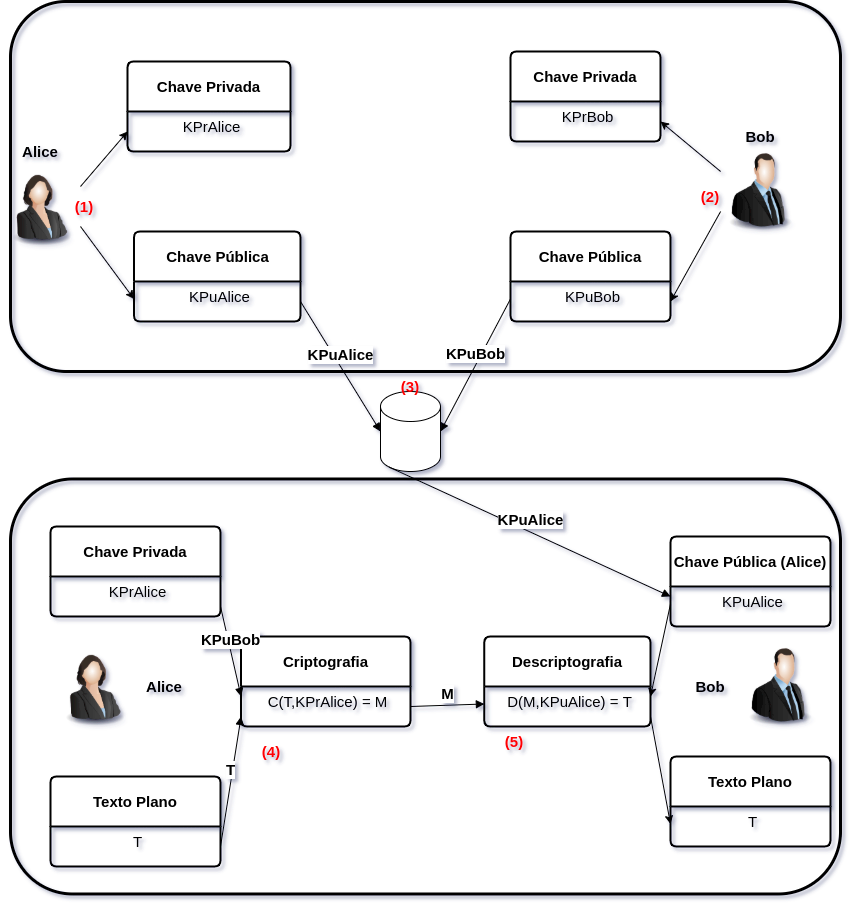
\includegraphics[scale=0.45]{assinatura.png}
	\caption{Funcionamento do processo de Assinatura Digital}
	\label{fig:assinatura}
\end{figure}

\pagebreak
